\documentclass[tikz,border=5pt]{standalone}
\usetikzlibrary{mindmap}
\begin{document}
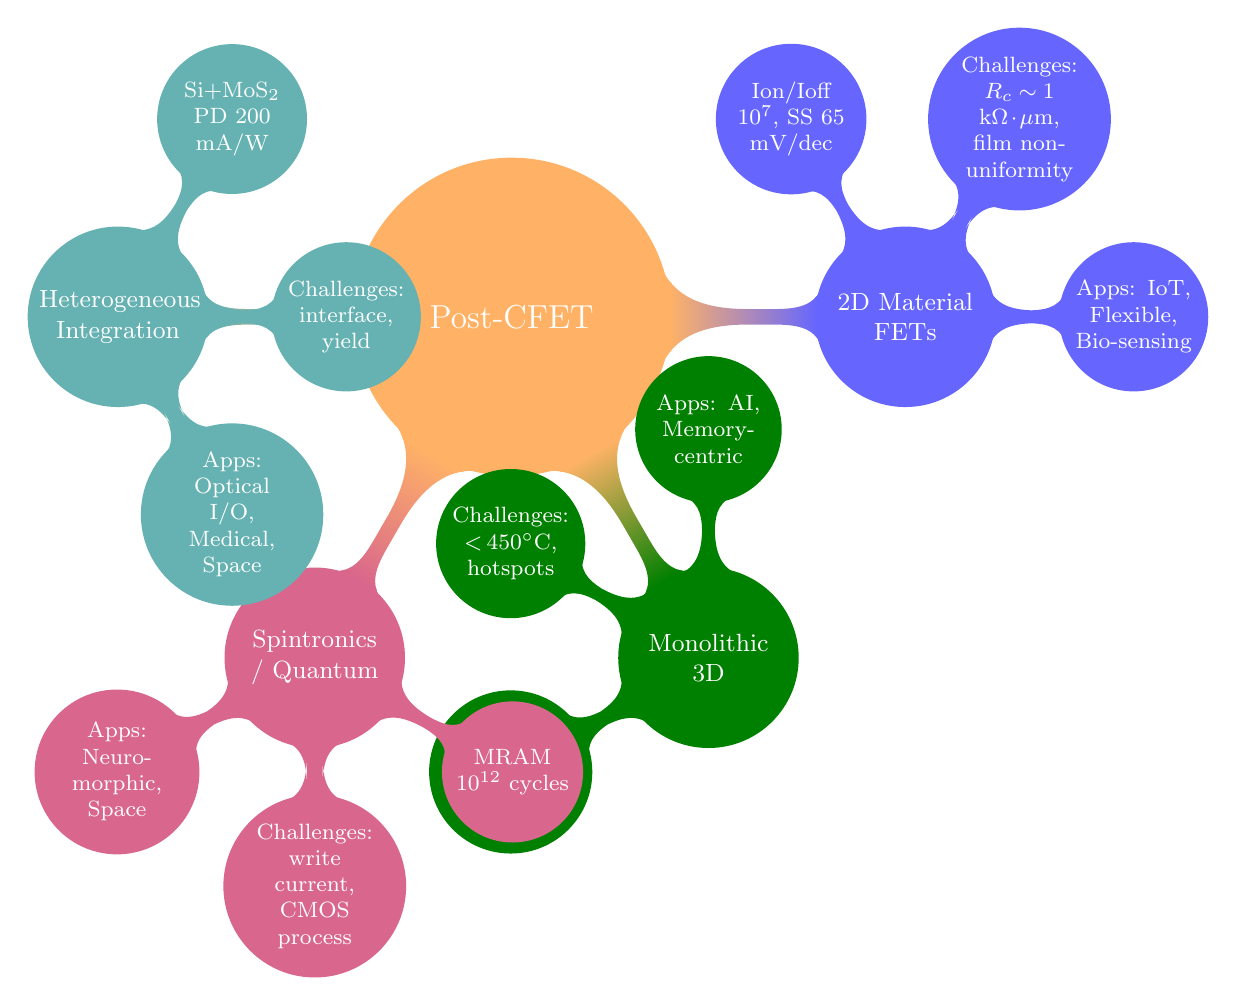
\begin{tikzpicture}
\path[mindmap,concept color=orange!60,text=white]
  node[concept] {Post-CFET}
    [clockwise from=0]
    child[concept color=blue!60] { node[concept] {2D Material FETs}
      [clockwise from=120]
        child { node[concept] {Ion/Ioff $10^7$, SS 65 mV/dec} }
        child { node[concept] {Challenges: $R_c\!\sim\!1$ k$\Omega\!\cdot\!\mu$m, film non-uniformity} }
        child { node[concept] {Apps: IoT, Flexible, Bio-sensing} }
    }
    child[concept color=green!50!black] { node[concept] {Monolithic 3D}
      [clockwise from=210]
        child { node[concept] {Delay $-30\%$, Area $-40\%$} }
        child { node[concept] {Challenges: $<\!450^{\circ}\mathrm{C}$, hotspots} }
        child { node[concept] {Apps: AI, Memory-centric} }
    }
    child[concept color=purple!60] { node[concept] {Spintronics / Quantum}
      [clockwise from=-30]
        child { node[concept] {MRAM $10^{12}$ cycles} }
        child { node[concept] {Challenges: write current, CMOS process} }
        child { node[concept] {Apps: Neuromorphic, Space} }
    }
    child[concept color=teal!60] { node[concept] {Heterogeneous Integration}
      [clockwise from=60]
        child { node[concept] {Si+MoS$_2$ PD 200 mA/W} }
        child { node[concept] {Challenges: interface, yield} }
        child { node[concept] {Apps: Optical I/O, Medical, Space} }
    };
\end{tikzpicture}
\end{document}
